We will distinguish between quantities that can be computed from information
already present during a traditional backward pass (which we suggestively call
\emph{first-order extensions}), and quantities that need additional information
(termed \emph{second-order extensions}). The former group contains additional
statistics such as the variance of the gradients within the mini-batch or the
$L_2$ norm of the gradient for each sample. Those can be computed with
minimal overhead during the backprop pass. The latter class contains
approximations of second-order information, like the diagonal or Kronecker
factorization of the generalized Gauss-Newton (\GGN) matrix, which require the
propagation of additional information through the graph. We will present those
two classes separately:

\begin{figure*}[!h]
  \centering
  \begin{minipage}[t]{0.495\linewidth}
    \begin{center}
      \textbf{First-order extensions}\\
      Extract more from the standard backward pass.~\\[-.75em]
      \begin{itemize}
      \item Individual gradients from a mini-batch
      \item $L_2$ norm of the individual gradients
      \item Diagonal covariance and 2\textsuperscript{nd} moment
      \end{itemize}
    \end{center}
  \end{minipage}
  \hfill
  \begin{minipage}[t]{0.495\linewidth}
    \begin{center}
      \textbf{Second-order extensions}\\
      Propagate new information along the graph.~\\[-.75em]
      \begin{itemize}
      \item Diagonal of the \GGN%
        and the Hessian
      \item \KFAC%
        \citep{martens2015optimizing}
      \item \KFRA%
        and \KFLR%
        \citep{botev2017practical}
      \end{itemize}
    \end{center}
  \end{minipage}
\end{figure*}

These quantities are only defined, or reasonable to compute, for a subset of
models: the concept of individual gradients for each sample in a mini-batch or
the estimate of the variance requires the loss for each sample to be
independent. While such functions are common in machine learning, not all neural
networks fit into this category. \Eg if the network uses batch normalization
\citep{ioffe2015batch}, the individual gradients in a mini-batch are correlated.
Then, the variance is not meaningful anymore, and computing the individual
contribution of a sample to the mini-batch gradient or the \GGN%
becomes prohibitive. For those reasons, and to limit the scope of the project
for version 1.0, \BackPACK%
currently restricts the type of models it accepts. The supported models are
traditional feedforward networks that can be expressed as a \emph{sequence of
  modules}, for example a sequence of convolutional, pooling, linear and
activation layers. Recurrent networks like \LSTM%
\!\!s \citep{hochreither1997lstm} or residual networks \citep{he2016deep} are
not yet supported, but the framework can be extended to cover them\sidenote{%
  \BackPACK has been continuously developed since the initial release.
  Noteworthy added features include:
  \begin{itemize}
  \item New extensions: per-sample Hessian/GGN diagonal (version 1.3),
    matrix-free multiplication with block-diagonal curvature matrices from
    \Cref{chap:hbp} (version 1.2), and \ggn low-rank factors (versions 1.4, 1.5),
    see \Cref{chap:vivit}.
  \item Broader support of modules and hyperparameters, especially basic support
    for residual and recurrent networks (version 1.4).
  \end{itemize}
}.

We assume a sequential model $f_{\vtheta}: \times \sX \rightarrow \sF$
and a dataset of $N$ samples $(\vx_n, \vy_n) \in \sX \times \sY$ with
$n=1,\dots, N$. The model maps each sample $\vx_n$ to a prediction
$f_{\vtheta}(\vx_n)$ using some parameters $\vtheta \in \sTheta$. The
predictions are evaluated with a loss function $\ell : \sF \times \sY
\rightarrow \R$, for example the softmax cross-entropy
(\Cref{eq:background::supervisedLearning}), which compares them to the ground
truth $\vy_n$. This leads to the objective function $\mathcal{L}: \sTheta
\rightarrow \R$,
\begin{equation}
  \label{backpack::eq:objective}
  \Loss(\vtheta)
  =
  \frac{1}{N} \sum_{n=1}^N \ell(f_{\vtheta}(\vx_n), \vy_n)\equationPunctuation{.}
\end{equation}
As a shorthand, we will use $\ell_n(\vtheta) = \ell(f_{\vtheta}(\vx_n), \vy_n)$
for the loss and $\vf_n(\vtheta) = f_{\vtheta}(\vx_n)$ for the model output of
individual samples. Our goal is to provide more information about the
derivatives of ${\{\ell_n(\vtheta)\}}_{n=1}^{N}$ \wrt the parameters
$\vtheta$ of the model $f_{\vtheta}$.

\subsection{Primer on Backpropagation}

ML libraries with integrated automatic differentiation use the
modular structure of $\vf_n(\vtheta)$ to compute derivatives
(see~\cite{baydin2018automatic} for an overview). If $f_{\vtheta}$ is a sequence
of $L$ transformations, it can be expressed as
\begin{equation}
  \vf_n(\vtheta)
  =
  \left(
    f^{(L)}_{\vtheta^{(L)}} \circ \ldots \circ f^{(1)}_{\vtheta^{(1)}}
  \right)(\vx_n)\equationPunctuation{,}
\end{equation}
where $f^{(l)}_{\vtheta^{(l)}}$ is the $l$th transformation with parameters
$\vtheta^{(l)}$, such that $\vtheta = ( \vtheta^{(1)\top}, \ldots, \vtheta^{(L)\top} )^{\top}$.
The loss function can also be seen as another transformation, appended to the
network. Let $\vz_n^{(l-1)}, \vz_n^{(l)}$ denote the input and output of the
operation $f^{(l)}_{\vtheta^{(l)}}$ for sample $n$, such that $\vz_n^{(0)}$ is
the original data and $\vz_n^{(1)}, \ldots, \vz_n^{(L)}$
represent the transformed output of each layer, leading to the computation graph\\[-.5em]
\[
  \textstyle \vz_n^{(0)}
  \stackrel{f^{(1)}_{\vtheta^{(1)}}(\vz_n^{(0)})}{\verylongrightarrow}
  \vz_n^{(1)}
  \stackrel{f^{(2)}_{\vtheta^{(2)}}(\vz_n^{(1)})}{\verylongrightarrow} \ldots
  \stackrel{f^{(L)}_{\vtheta^{(L)}}(\vz_n^{(L-1)})}{\verylongrightarrow}
  \vz_n^{(L)} \stackrel{\ell(\vz_n^{(L)}, \vy_n)}{\verylongrightarrow}
  \ell_n(\vtheta)\equationPunctuation{.}
\]
To compute the gradient of $\ell_n$ \wrt $\vtheta^{(l)}$, one unrolls the chain rule,
\begin{equation}
  \begin{split}
    \grad{\vtheta^{(l)}} \ell_n(\vtheta)
    &=
      {\left(\jac_{\vtheta^{(l)}}
      \vz_n^{(l)}\right)}^\top
      {\left(\jac_{\vz_n^{(l)}} \vz_n^{(l+1)}\right)}^\top
      \cdots
      {\left(\jac_{\vz_n^{(L-1)}} \vz_n^{(L)}\right)}^\top
      \grad{\vz_n^{(L)}}\ell_n(\vtheta)
    \\
    &=
      {\left(\jac_{\vtheta^{(l)}} \vz_n^{(l)}\right)}^\top
      \grad{\vz^{(l)}}\ell_n(\vtheta)\equationPunctuation{,}
  \end{split}\label{backpack::eq:backprop_gradient}
\end{equation}
where $\jac_{\va} \vb$ is the Jacobian of $\vb$ \wrt $\va$, ${[\jac_{\va}
  \vb]}_{i,j} = \partial {[\vb]}_i / \partial {[\va]}_j$ (see
\Cref{def:background::JacobianVectorVector}). A similar expression exists for
the module inputs $\vz_n^{(l-1)}$: $ \grad{\vz_n^{(l-1)}}\ell_n(\vtheta) =
(\jac_{\vz_n^{(l-1)}} \vz_n^{(l)})^\top \grad{\vz_n^{(l)}}\ell_n(\vtheta). $
This recursive structure makes it possible to extract the gradient by
propagating the gradient of the loss. In the backpropagation algorithm, a module
$l$ receives the loss gradient \wrt its output,
$\grad{\vz_n^{(l)}}\ell_n(\vtheta)$. It then extracts the gradient with respect
to its parameters and inputs, $\grad{\vtheta^{(l)}}\ell_n(\vtheta)$ and
$\grad{\vz_n^{(l-1)}}\ell_n(\vtheta)$, according to
\Cref{backpack::eq:backprop_gradient}. The gradient \wrt its input is sent
further down the graph. This process, illustrated in
\Cref{backpack::fig:backprop-gradient}, is repeated for each transformation
until all gradients are computed. To implement backpropagation, each module only
needs to know how to multiply with its Jacobians.

\begin{figure}[!t]
  \centering
  \tikzexternalenable%
  \begin{tikzpicture}
  \definecolor{lightGray}{HTML}{b3b3b3}
  \pgfmathsetmacro{\figureWidthPt}{\linewidth}

  \node (im) [inner sep=0pt] {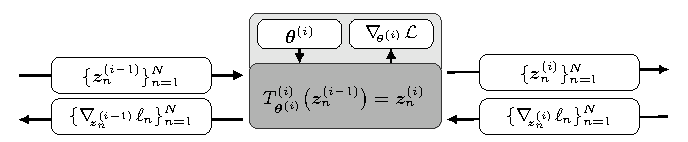
\includegraphics[width=\figureWidthPt pt]{../repos/backpack-paper/tex/paper/figs/backprop-modules/vanilla_backprop.pdf}};

  \newcommand{\relativeCoordinate}[2]{($(im.south west)!#1!(im.south east)+(im.south west)!#2!(im.north west)-(im.south west)$)}

  % bottom left
  \node [rectangle, fill=white, draw=none, inner sep=0pt, minimum height =
  0.04*\figureWidthPt pt, minimum width = 0.18*\figureWidthPt pt, anchor=center]
  at \relativeCoordinate{0.19}{0.18} {$\{ \grad{\vz_n^{(l-1)}}\ell_n \}_n$};

  % top left
  \node [rectangle, fill=white, draw=none, inner sep=0pt, minimum height =
  0.04*\figureWidthPt pt, minimum width = 0.18*\figureWidthPt pt, anchor=center]
  at \relativeCoordinate{0.19}{0.47} {$\{ \vz_n^{(l-1)}\}_n$};

  % bottom right
  \node [rectangle, fill=white, draw=none, inner sep=0pt, minimum height =
  0.04*\figureWidthPt pt, minimum width = 0.18*\figureWidthPt pt, anchor=center]
  at \relativeCoordinate{0.81}{0.18} {$\{ \grad{\vz_n^{(l)}}\ell_n \}_n$};

  % top right
  \node [rectangle, fill=white, draw=none, inner sep=0pt, minimum height =
  0.04*\figureWidthPt pt, minimum width = 0.18*\figureWidthPt pt, anchor=center]
  at \relativeCoordinate{0.81}{0.49} {$\{ \vz_n^{(l)}\}_n$};

  % center left
  \node [rectangle, fill=white, draw=none, inner sep=0pt, minimum height =
  0.035*\figureWidthPt pt, minimum width = 0.1*\figureWidthPt pt, anchor=center]
  at \relativeCoordinate{0.435}{0.76} {$\vtheta^{(l)}$};

  % center right
  \node [rectangle, fill=white, draw=none, inner sep=0pt, minimum height =
  0.035*\figureWidthPt pt, minimum width = 0.1*\figureWidthPt pt, anchor=center]
  at \relativeCoordinate{0.5685}{0.76} {$\grad{\vtheta^{(l)}}\gL$};

  % module
  \node [rectangle, fill=lightGray, draw=none, inner sep=0pt, minimum height =
  0.07*\figureWidthPt pt, minimum width = 0.25*\figureWidthPt pt, anchor=center]
  at \relativeCoordinate{0.5}{0.33} {$f_{\vtheta^{(l)}}^{(l)}$};
\end{tikzpicture}
%%% Local Variables:
%%% mode: latex
%%% TeX-master: "../../thesis"
%%% End:

  \tikzexternaldisable%
  \caption{\textbf{Schematic representation of the standard backpropagation
      pass} for module $l$ with $N$
    samples.}\label{backpack::fig:backprop-gradient}
\end{figure}

For second-order quantities, we rely on the work of
\citet{mizutani2008secondorder} and \citet{dangel2020modular}, who showed that a
scheme similar to \Cref{backpack::eq:backprop_gradient} exists for the
\emph{block diagonal} of the Hessian. A block \wrt the parameters of
a module, $\gradsquared{\vtheta^{(l)}}\ell_n(\vtheta)$, can be obtained by the
recursion
\begin{equation}
  \begin{split}
    \gradsquared{\vtheta^{(l)}}\ell_n(\vtheta)
    &=
    {\left(\jac_{\vtheta^{(l)}} \vz_n^{(l)}\right)}^\top
    \gradsquared{\vz_n^{(l)}}\ell_n(\vtheta)
    \left(\jac_{\vtheta^{(l)}} \vz_n^{(l)}\right)
    \\
    &\phantom{=}\
    + \sum_j
    \left(\gradsquared{\vtheta^{(l)}} {\left[\vz_n^{(l)}\right]}_j\right)
    {\left[ \grad{\vz_n^{(l)}}\ell_n(\vtheta) \right]}_j\equationPunctuation{.}
  \end{split}
  \label{backpack::eq:backprop_hessian}
\end{equation}
A similar relation holds for the module's output Hessian
$\gradsquared{\vz_n^{(l)}} \ell_n(\vtheta)$.

Both backpropagations of
\Cref{backpack::eq:backprop_gradient,backpack::eq:backprop_hessian} hinge on the
multiplication by Jacobians to both vectors and matrices. However, the design of
AD limits the application of Jacobians to vectors only. This prohibits the
exploitation of vectorization in the matrix case, which is needed for
second-order information. The lacking flexibility of Jacobians is one motivation
for our work. Since all quantities needed to compute statistics of the
derivatives are already computed during the backward pass, another motivation is
to provide access to them at minor overhead.

\subsection{First-order Extensions}
As the principal first-order extension, consider computing the \emph{per-sample}
gradients in a batch of size $N$. These individual gradients are implicitly
computed during a traditional backward pass because the batch gradient is their
sum, but they are not directly accessible. The naïve way to compute $N$
individual gradients is to do $N$ separate forward and backward passes, This
(inefficiently) replaces every matrix-matrix multiplication by $N$ matrix-vector
multiplications. \BackPACK batches computations to obtain large efficiency
gains, as illustrated by
\Cref{backpack::fig:bench-individual-gradients}\sidenote{%
  The latest developments in ML libraries have lead to more efficient
  alternatives than the for-loop. \pytorch 1.11.0 (released on March 10, 2022)
  introduced an \inlinecode{is\_grads\_batched} argument in the API of
  the
  \href{https://pytorch.org/docs/1.11/generated/torch.autograd.grad.html}{\inlinecode{grad}}
  function of
  its \href{https://pytorch.org/docs/1.11/autograd.html}{\inlinecode{autograd}}
  library, which allows to compute multiple VJPs in parallel. This reflects the
  importance of the feature.}.

\begin{figure}
  \centering
  \pgfkeys{/pgfplots/BackPACKBenchBarplot/.style={
    width=1.02\linewidth,
    height=0.5\linewidth,
    grid=major,
    grid style = {dashed},
    every axis plot/.append style={line width = 1.5pt},
    tick pos = left,
    xtick align = outside,
    ytick align = inside,
    xmajorticks = true,
    ymajorticks = true,
    ylabel near ticks,
    xlabel near ticks,
    xticklabel style = {font = \footnotesize},
    xlabel style = {font = \footnotesize},
    axis line style = {black},
    yticklabel style = {font = \footnotesize},
    ylabel style = {font = \footnotesize},
    title style = {font = \footnotesize, inner ysep = 0ex},
    grid = major,
    grid style = {dashed},
    legend cell align = left,
    legend style = {
      fill opacity = 0.7,
      text opacity = 1,
      font = \footnotesize,
      legend columns = 4,
      legend cell align={left},
      legend image post style={opacity = 1, yscale = 1.1, line width=-1pt},
      column sep=0.25cm,
    },
  }
}

%%% Local Variables:
%%% mode: latex
%%% TeX-master: "../../thesis"
%%% End:

  \pgfkeys{/pgfplots/zmystyle/.style={
      BackPACKBenchBarplot
    }
  }
  \tikzexternalenable%
  % This file was created by tikzplotlib v0.9.7.
\begin{tikzpicture}

\definecolor{color0}{rgb}{0.211764705882353,0.294117647058824,0.603921568627451}
\definecolor{color1}{rgb}{0.431372549019608,0.650980392156863,0.803921568627451}
\definecolor{color2}{rgb}{0.76078431372549,0.894117647058824,0.937254901960784}

\begin{axis}[
legend cell align={left},
legend style={fill opacity=0.8, draw opacity=1, text opacity=1, draw=white!80!black},
tick align=outside,
tick pos=left,
title={Batch gradients},
x grid style={white!69.0196078431373!black},
xmin=-0.5125, xmax=2.5125,
xtick style={color=black},
xtick={0,1,2},
xticklabels={For-loop,BackPACK,Gradient
(Ref.)},
y grid style={white!69.0196078431373!black},
ylabel={Time [ms]},
ymin=0, ymax=715.401721642411,
ytick style={color=black},
zmystyle
]
\draw[draw=none,fill=white!20!black] (axis cs:1.625,0) rectangle (axis cs:1.875,22.247069500736);
\draw[draw=none,fill=color0] (axis cs:-0.375,0) rectangle (axis cs:-0.125,190.67248400097);
\addlegendimage{ybar,ybar legend,draw=none,fill=color0};
\addlegendentry{Batch size 64}

\draw[draw=none,fill=color0] (axis cs:0.625,0) rectangle (axis cs:0.875,30.771913996432);
\draw[draw=none,fill=white!40!black] (axis cs:1.875,0) rectangle (axis cs:2.125,40.6486490028328);
\draw[draw=none,fill=color1] (axis cs:-0.125,0) rectangle (axis cs:0.125,367.899422002665);
\addlegendimage{ybar,ybar legend,draw=none,fill=color1};
\addlegendentry{                 128}

\draw[draw=none,fill=color1] (axis cs:0.875,0) rectangle (axis cs:1.125,57.7847249951446);
\draw[draw=none,fill=color2] (axis cs:0.125,0) rectangle (axis cs:0.375,681.334972992772);
\addlegendimage{ybar,ybar legend,draw=none,fill=color2};
\addlegendentry{                 256}

\draw[draw=none,fill=color2] (axis cs:1.125,0) rectangle (axis cs:1.375,96.5649990030215);
\draw[draw=none,fill=white!60!black] (axis cs:2.125,0) rectangle (axis cs:2.375,79.2037880019052);
\addplot [semithick, white!20!black, opacity=0.4, forget plot]
table {%
-0.5125 22.247069500736
2.5125 22.247069500736
};
\addplot [semithick, white!40!black, opacity=0.4, forget plot]
table {%
-0.5125 40.6486490028329
2.5125 40.6486490028329
};
\addplot [semithick, white!60!black, opacity=0.4, forget plot]
table {%
-0.5125 79.2037880019052
2.5125 79.2037880019052
};
\end{axis}

\end{tikzpicture}

  \tikzexternaldisable%
  \caption{\textbf{Computing individual gradients in a batch using a for-loop
      (\ie one individual forward and backward pass per sample) or using
      vectorized operations with \BackPACK.} The plot shows computation time,
    comparing to a traditional gradient computation, on the \CIFARTENNET%
    network (see \Cref{backpack::sec:experiments}) for the \CIFARTEN%
    dataset \citep{schneider2019deepobs}.
  }\label{backpack::fig:bench-individual-gradients}
\end{figure}

As the quantities necessary to compute the individual gradients are already
propagated through the computation graph, we can reuse them by inserting code in
the standard backward pass. With access to this information, before it is
cleared for memory efficiency, \BackPACK%
computes the Jacobian-multiplications
for each sample
\begin{equation}
  {\left\{
      \grad{\vtheta^{(l)}} \ell_n(\vtheta)
    \right\}}_{n=1}^N
  =
  {\left\{
      {\left(\jac_{\vtheta^{(l)}} \vz^{(l)}_n\right)}^\top \grad{\vz_n^{(l)}} \ell_n(\vtheta)
    \right\}}_{n=1}^N\equationPunctuation{,}
\end{equation}
without summing the result---see \Cref{backpack::fig:first-order-extraction} for
a schematic representation. This duplicates some of the computation performed by
the backpropagation, as the Jacobian is applied twice (once by \PyTorch%
and \BackPACK%
with and without summation over the samples, respectively). However, the
associated overhead is small compared to the for-loop approach: the major
computational cost arises from the propagation of information required for each
layer, rather than the formation of the gradient \emph{within} each layer.

This scheme for individual gradient computation is the basis for all first-order
extensions. In this direct form, however, it is expensive in memory: if the
model is $D$-dimensional, storing $\gO(ND)$ elements is prohibitive for large
batches. For the variance, 2\textsuperscript{nd} moment and $L_2$ norm,
\BackPACK%
takes advantage of the Jacobian's structure to directly compute them without
forming the individual gradient, reducing memory overhead. See
\Cref{backpack::app:first-order-extensions} for details.

\begin{figure}[!t]
  \centering
  \tikzexternalenable%
  \begin{tikzpicture}
  \definecolor{lightBlue}{HTML}{d1e5f0}
  \definecolor{lightGray}{HTML}{b3b3b3}
  \pgfmathsetmacro{\figureWidthPt}{\linewidth}

  \node (im) [inner sep=0pt] {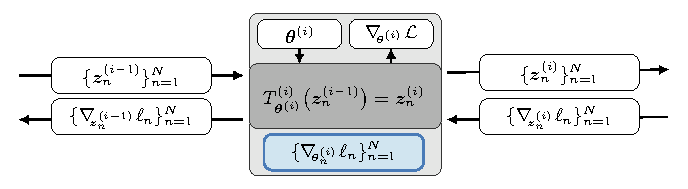
\includegraphics[width=\figureWidthPt pt]{../repos/backpack-paper/tex/paper/figs/backprop-modules/indiv_grad.pdf}};

  \newcommand{\relativeCoordinate}[2]{($(im.south west)!#1!(im.south east)+(im.south west)!#2!(im.north west)-(im.south west)$)}

  % bottom left
  \node [rectangle, fill=white, draw=none, inner sep=0pt, minimum height =
  0.04*\figureWidthPt pt, minimum width = 0.18*\figureWidthPt pt, anchor=center]
  at \relativeCoordinate{0.19}{0.385} {$\{ \grad{\vz_n^{(l-1)}}\ell_n \}_n$};

  % top left
  \node [rectangle, fill=white, draw=none, inner sep=0pt, minimum height =
  0.04*\figureWidthPt pt, minimum width = 0.18*\figureWidthPt pt, anchor=center]
  at \relativeCoordinate{0.19}{0.6} {$\{ \vz_n^{(l-1)}\}_n$};

  % bottom right
  \node [rectangle, fill=white, draw=none, inner sep=0pt, minimum height =
  0.04*\figureWidthPt pt, minimum width = 0.18*\figureWidthPt pt, anchor=center]
  at \relativeCoordinate{0.81}{0.385} {$\{ \grad{\vz_n^{(l)}}\ell_n \}_n$};

  % top right
  \node [rectangle, fill=white, draw=none, inner sep=0pt, minimum height =
  0.04*\figureWidthPt pt, minimum width = 0.18*\figureWidthPt pt, anchor=center]
  at \relativeCoordinate{0.81}{0.615} {$\{ \vz_n^{(l)}\}_n$};

  % center left
  \node [rectangle, fill=white, draw=none, inner sep=0pt, minimum height =
  0.03*\figureWidthPt pt, minimum width = 0.1*\figureWidthPt pt, anchor=center]
  at \relativeCoordinate{0.435}{0.82} {$\vtheta^{(l)}$};

  % center right
  \node [rectangle, fill=white, draw=none, inner sep=0pt, minimum height =
  0.03*\figureWidthPt pt, minimum width = 0.1*\figureWidthPt pt, anchor=center]
  at \relativeCoordinate{0.5685}{0.82} {$\grad{\vtheta^{(l)}}\gL$};

  % module
  \node [rectangle, fill=lightGray, draw=none, inner sep=0pt, minimum height =
  0.05*\figureWidthPt pt, minimum width = 0.25*\figureWidthPt pt, anchor=center]
  at \relativeCoordinate{0.5}{0.49} {$f_{\vtheta^{(l)}}^{(l)}$};

  % center bottom
  \node [rectangle, fill=lightBlue, draw=none, inner sep=0pt, minimum height =
  0.04*\figureWidthPt pt, minimum width = 0.2*\figureWidthPt pt, anchor=center]
  at \relativeCoordinate{0.5}{0.195} {$\{ \grad{\vtheta^{(l)}} \ell_n\}_n$};
\end{tikzpicture}
%%% Local Variables:
%%% mode: latex
%%% TeX-master: "../../thesis"
%%% End:

  \tikzexternaldisable%
  \caption{\textbf{Schematic representation of the individual gradients'
      extraction in addition to the standard backward pass} at the $l$th module
      for $N$ samples.}\label{backpack::fig:first-order-extraction}
\end{figure}

\subsection{Second-order Extensions}\label{backpack::sec:backpack-second-order}
Second-order extensions require propagation of more information through the
graph. %
\marginnote[*-20]{
  \begin{example}[\textbf{Symmetric decomposition of the softmax cross-entropy loss
    Hessian~\cite{papyan2019measurements}}]\label{ex:backpack::symmetricDecompositionCE}
  Consider the softmax cross-entropy loss
  (\Cref{eq:background::softmaxCrossEntropyLoss}) Hessian from Table
  \Cref{hbp::table:backpropEquations}. Its symmetric decomposition $\mS \in
  \sR^{C\times C}$ is
    \begin{align}
      \label{eq:backpack::sqrtCrossEntropyLoss}
      \begin{split}
        \mS
        &=
          \left(
          \mI - \vp\,\vone^{\top}
          \right)
          \diag\left( \sqrt{\vp} \right)
        \\
        &=
          \diag\left( \sqrt{\vp} \right)
          -
          \vp \sqrt{\vp}^{\top}\,,
      \end{split}
    \end{align}
    where $\sqrt{\vp(\vf)} = {\vp(\vf)}^{\odot \nicefrac{1}{2}}$. It satisfies
    $\gradsquared{\vf}\ell(\vf, \vy) = \mS \mS^{\top}$,
    \begin{align*}
      \mS \mS^{\top}
      &=
        \left[
        \diag\left( \sqrt{\vp} \right)
        -
        \vp \sqrt{\vp}^{\top}\,
        \right]
      \\
      &\phantom{= \ }
        \left[
        \diag\left( \sqrt{\vp} \right)
        -
        \sqrt{\vp} \vp^{\top}\,
        \right]
      \\
      &=
        \diag\left( \vp \right)
        - 2 \vp \vp^{\top}
        + \vp \sqrt{\vp}^{\top}
        \sqrt{\vp} \vp^{\top}
      \\
      &=
        \diag\left( \vp \right)
        - \vp \vp^{\top}\,,
    \end{align*}
    using that $\vp$'s elements sum to one, \ie $\sqrt{\vp}^{\top}\sqrt{\vp} =
    1$. This is the expression from \Cref{hbp::table:backpropEquations}.
  \end{example}
}%
As an example, we will focus on the \GGN matrix
\citep{schraudolph2002fast}. It is guaranteed to be PSD and is a reasonable
approximation of the Hessian near the minimum, which motivates its use in
approximate second-order methods. For popular loss functions, it coincides with
the Fisher information matrix used in natural gradient methods
\citep{amari1998natural}; for a more in depth discussion of the equivalence, see
\Cref{sec:background::naturalGradientDescent} and the reviews of
\citet{martens2014new} and \citet{kunstner2019limitations}. For an objective
function that can be written as the composition of a loss function $\ell$ and a
model $f_{\vtheta}$, such as \Cref{backpack::eq:objective}, the \GGN%
of $\nicefrac{1}{N} \sum_n \ell(f_{\vtheta}(\vx_n), \vy_n)$ is
\begin{equation}
  \label{backpack::eq:main-ggn}
  \mG(\vtheta) =
  \frac{1}{N} \sum_n
  {\left(\jac_\vtheta \vf_n \right)}^\top
  \gradsquared{\vf_n} \ell(\vf_n, \vy_n) \:
  \left(\jac_\vtheta \vf_n\right)\equationPunctuation{.}
\end{equation}
\marginnote[*-10]{%
  \begin{example}[\textbf{\mc approximation of the softmax-cross entropy loss
    Hessian}]\label{ex:backpack::symmetricMCDecompositionCE} Consider the softmax
  cross-entropy loss (\Cref{eq:background::softmaxCrossEntropyLoss}) Hessian
  from \Cref{hbp::table:backpropEquations}. An \mc approximation of the
  symmetric decomposition (\Cref{eq:backpack::sqrtCrossEntropyLoss}) is
  constructed by the vectors
    \begin{align}
      \label{equ:backpack::sqrtMCVectorsCrossEntropyLoss}
      \vstilde = \vytilde(c) - \vp(\vf)
    \end{align}
    with $\vytilde(c) = \onehot(c)$ and $c$ drawn from a categorical
    distribution implied by the softmax-probabilities, $c \sim \Cat(c;
    \vp(\vf))$. The random vector $\vytilde$ satisfies $\E_{c}\left[ \vytilde
    \right] = \vp(\vf)$ and $\E_{c}\left[ \vytilde \vytilde^{\top} \right] =
    \diag[\vp(\vf)]$. With these properties, we can show
    $\E_{\vstilde}\left[\vstilde\vstilde^{\top}\right] = \gradsquared{\vf}\ell$,
    \ie%
    the expected outer product of
    \Cref{equ:backpack::sqrtMCVectorsCrossEntropyLoss} is the Hessian,
    \begin{align*}
      \E_{\vstilde} \left[\vstilde \vstilde^{\top}\right]
      &=
        \E_{c}[ \vytilde \vytilde^{\top} ]
        - \E_{c}[ \vytilde]  \vp^{\top}
      \\
      &\phantom{= \,}
        -  \vp \E_{c}[\vytilde^{\top} ]
        + \vp \vp^{\top}
      % \\
      % &=
      %   \diag(\vp) - 2 \vp \vp^{\top} + \vp\vp^{\top}
      \\
      &=
        \diag(\vp) - \vp \vp^{\top}\,.
    \end{align*}
    Instead of using the $C \times C$ matrix square root $\mS$, we can draw $M <
    C$ samples $c_1, \dots, c_M$ and stack their $\vstilde$-vectors into a
    smaller $C \times M $ matrix
    \begin{align}
      \mStilde
      =
      \frac{1}{\sqrt{M}}
      \begin{pmatrix}
        \vstilde(c_1)\  \dots\  \vstilde(c_M)
      \end{pmatrix}
    \end{align}
    that approximates \Cref{eq:backpack::sqrtCrossEntropyLoss},
    \begin{align*}
      \mStilde \mStilde^{\top}
      &=
        \frac{1}{M}
        \sum_{i=1}^{M}
        \vstilde(c_i)
        {\vstilde(c_i)}^{\top}
      \\
      &\approx \E_{\vstilde}\left[ \vstilde \vstilde^{\top}\right]
        = \mS \mS^{\top}\,,
    \end{align*}
    using less memory. From the connection between Fisher and Hessian,
    \Cref{equ:backpack::sqrtMCVectorsCrossEntropyLoss} are `would-be gradients'
    under targets sampled from the model's likelihood, \ie%
    $\vstilde^{\top} = \jac_{\vf}\ell(\vf, \vytilde)$ with $\vytilde \sim
    q(\giventhat{\cdot}{\vf})$ and the Jacobian from
    \Cref{tab:background::Jacobians}.
  \end{example}
}%
The full matrix is too large to compute and store. Current approaches focus on
its diagonal blocks, where each block corresponds to a layer in the network.
Every block itself is further approximated, for example using a Kronecker
factorization. The approach used by \BackPACK%
for their computation is a refinement of the \emph{Hessian Backpropagation
  equations} of \citet{dangel2020modular}. It relies on two insights: firstly,
the computational bottleneck in the \ggn's computation is the multiplication
with the Jacobian of the network, $\jac_\vtheta \vf_n$, while the network output
Hessian is easy to compute for most popular loss functions. Secondly, it is not
necessary to compute and store each of the $N$ $D \times D$ matrices for a
network with $D$ parameters, as \Cref{backpack::eq:main-ggn} is a quadratic
expression. Given a symmetric factorization $\mS_n$ of the Hessian,
$\mS_n\mS_n^\top = \gradsquared{\vf_n} \ell(\vf_n, \vy_n)$ (\eg
\Cref{ex:backpack::symmetricDecompositionCE}), it is sufficient to compute
${(\jac_\vtheta \vf_n)}^\top \mS_n$ and square the result. A network output is
typically small compared to its inner layers; networks on \CIFARHUN%
need $C=100$ class outputs but could use convolutional layers with more than
100,000 parameters.

The factorization leads to a $D \times C$ matrix, which makes it possible to
efficiently compute \GGN%
block diagonals. Also, the computation is very similar to that of a gradient,
which computes ${(\jac_\vtheta \vf_n)}^\top \grad{\vf_n} \ell_n$. A module
$f^{(l)}_{\vtheta^{(l)}}$ receives the symmetric factorization of the \GGN%
\wrt its output, $\vz^{(l)}_n$, and multiplies it with the Jacobians
\wrt the parameters $\vtheta^{(l)}$ and inputs $\vz^{(l-1)}_n$ to
produce a symmetric factorization of the \GGN%
\wrt the parameters and inputs, as shown in
\Cref{backpack::fig:second-order-pass}.

\begin{figure}[!t]
  \centering
  \tikzexternalenable%
  \begin{tikzpicture}
  \definecolor{lightBlue}{HTML}{d1e5f0}
  \definecolor{lightGray}{HTML}{b3b3b3}
  \pgfmathsetmacro{\figureWidthPt}{\linewidth}

  \node (im) [inner sep=0pt] {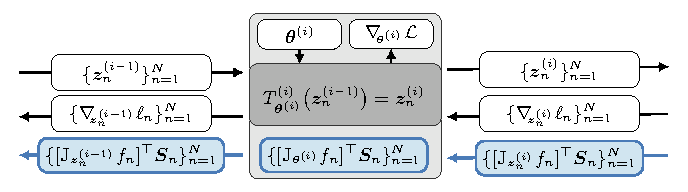
\includegraphics[width=\figureWidthPt pt]{../repos/backpack-paper/tex/paper/figs/backprop-modules/second_order.pdf}};

  \newcommand{\relativeCoordinate}[2]{($(im.south west)!#1!(im.south east)+(im.south west)!#2!(im.north west)-(im.south west)$)}

  % bottom left
  \node [rectangle, fill=lightBlue, draw=none, inner sep=0pt, minimum height =
  0.04*\figureWidthPt pt, minimum width = 0.245*\figureWidthPt pt, anchor=center]
  at \relativeCoordinate{0.19}{0.195} {$\{ {(\jac_{\vz_n^{(l-1)}} \vf_n)}^{\top} \mS_n \}_n$};

  % center left
  \node [rectangle, fill=white, draw=none, inner sep=0pt, minimum height =
  0.04*\figureWidthPt pt, minimum width = 0.18*\figureWidthPt pt, anchor=center]
  at \relativeCoordinate{0.19}{0.41} {$\{ \grad{\vz_n^{(l-1)}}\ell_n \}_n$};

  % top left
  \node [rectangle, fill=white, draw=none, inner sep=0pt, minimum height =
  0.04*\figureWidthPt pt, minimum width = 0.18*\figureWidthPt pt, anchor=center]
  at \relativeCoordinate{0.19}{0.625} {$\{ \vz_n^{(l-1)}\}_n$};

  % bottom right
  \node [rectangle, fill=lightBlue, draw=none, inner sep=0pt, minimum height =
  0.04*\figureWidthPt pt, minimum width = 0.225*\figureWidthPt pt, anchor=center]
  at \relativeCoordinate{0.814}{0.18} {$\{ {(\jac_{\vz_n^{(l)}} \vf_n)}^{\top} \mS_n \}_n$};

  % center right
  \node [rectangle, fill=white, draw=none, inner sep=0pt, minimum height =
  0.04*\figureWidthPt pt, minimum width = 0.18*\figureWidthPt pt, anchor=center]
  at \relativeCoordinate{0.81}{0.41} {$\{ \grad{\vz_n^{(l)}}\ell_n \}_n$};

  % top right
  \node [rectangle, fill=white, draw=none, inner sep=0pt, minimum height =
  0.04*\figureWidthPt pt, minimum width = 0.18*\figureWidthPt pt, anchor=center]
  at \relativeCoordinate{0.81}{0.64} {$\{ \vz_n^{(l)}\}_n$};

  % center left
  \node [rectangle, fill=white, draw=none, inner sep=0pt, minimum height =
  0.03*\figureWidthPt pt, minimum width = 0.1*\figureWidthPt pt, anchor=center]
  at \relativeCoordinate{0.435}{0.82} {$\vtheta^{(l)}$};

  % center right
  \node [rectangle, fill=white, draw=none, inner sep=0pt, minimum height =
  0.03*\figureWidthPt pt, minimum width = 0.1*\figureWidthPt pt, anchor=center]
  at \relativeCoordinate{0.5685}{0.82} {$\grad{\vtheta^{(l)}}\gL$};

  % module
  \node [rectangle, fill=lightGray, draw=none, inner sep=0pt, minimum height =
  0.05*\figureWidthPt pt, minimum width = 0.25*\figureWidthPt pt, anchor=center]
  at \relativeCoordinate{0.5}{0.49} {$\vf_{\vtheta^{(l)}}^{(l)}$};

  % center bottom
  \node [rectangle, fill=lightBlue, draw=none, inner sep=0pt, minimum height =
  0.04*\figureWidthPt pt, minimum width = 0.22*\figureWidthPt pt, anchor=center]
  at \relativeCoordinate{0.5}{0.195} {$\{ {(\jac_{\vtheta^{(l)}} \vf_n)}^{\top} \mS_n \}_n$};
\end{tikzpicture}
%%% Local Variables:
%%% mode: latex
%%% TeX-master: "../../thesis"
%%% End:

  \tikzexternaldisable%
  \caption{\textbf{Schematic of the additional backward pass} to compute a
    symmetric factorization of the \GGN,
    \begin{align*}
      \mG(\vtheta) = \frac{1}{N} \sum_n {\left(\jac_{\vtheta} \vf_n\right)}^\top \mS_n \mS_n^\top
      \left(\jac_{\vtheta} \vf_n\right)
    \end{align*}
    alongside the gradient at the $l$th module, for $N$ samples.
  }\label{backpack::fig:second-order-pass}
\end{figure}

This propagation serves as the basis of the second-order extensions. If the full
symmetric factorization is not wanted, for memory reasons, it is possible to
extract more specific information such as the diagonal. If $\mB$ is the
symmetric factorization for a \GGN%
block, the diagonal can be computed as $[\diag(\mB\mB^\top)]_{i} =
{[\mB\mB^\top]}_{i,i} = \sum_j {[\mB]}_{i,j}^2$.

This framework can be used to extract the main Kronecker factorizations of the
\GGN, \KFAC%
and \KFLR, which we extend to convolution using the approach of
\citet{grosse2016kronecker}. The important difference between the two methods is
the initial matrix factorization $\mS_n$. Using a full symmetric factorization
of the initial Hessian, $\mS_n\mS_n^\top = \gradsquared{\vf_n}\ell_n$, yields
the \KFLR%
approximation. \KFAC%
uses an \MC approximation by sampling a vector $\vs_n$ such that
$\mathbb{E}_{\vs_n}[\vs_n\vs_n^\top] = \gradsquared{\vf_n} \ell_n$ (see
\Cref{ex:backpack::symmetricMCDecompositionCE}). \KFLR%
is therefore more precise but more expensive than \KFAC, especially for networks
with high-dimensional outputs, which is reflected in our benchmark on \CIFARHUN%
in \Cref{backpack::sec:benchmark}. The technical details on how Kronecker
factors are extracted and information is propagated for second-order \BackPACK%
extensions are documented in \Cref{backpack::app:second-order-extensions}.

%%% Local Variables:
%%% mode: latex
%%% TeX-master: "../thesis"
%%% End:
